\section{Desarrollo del Proyecto}

En esta sección explicaremos como ha sido desarrollado el proyecto, empezando por el Análisis de Exploración de Datos (EDA); el planteamiento de la arquitectura, donde se verán las decisiones tomadas para la construcción del modelo; la construcción del modelo; y las iteraciones de desarrollo.

\subsection{Análisis de Exploración de Datos}

El conjunto de datos utilizado procede de registros de partidas de Tenhou recopilados mediante la herramienta \textit{phoenix-logs} y transformados a una base de datos SQLite mediante \textit{tenhou\_dataprocess}. El dataset se distribuye a través de Kaggle con licencia Apache 2.0 y contiene ocho tablas asociadas a diferentes tipos de decisiones: \textit{Discard}, \textit{Riichi}, \textit{Chi}, \textit{Pon}, \textit{DaiMinKan}, \textit{ShouMinKan}, \textit{AnKan} y \textit{Skip}. Cada registro almacena un estado de juego serializado en formato JSON y comprimido mediante gzip.

En este proyecto se utiliza exclusivamente la tabla \textit{Discard}. A partir de ella se construyó una base de datos filtrada que conserva únicamente los estados con más de una alternativa de descarte, obteniéndose un total de 552.563 estados.

\begin{table}[H]
  \centering
  \caption{Schemas del Dataset}
  \label{tab:schemas}
  \begin{tabular}{@{}cll@{}}
    \toprule
    \textbf{ID} & \textbf{Nombre} & \textbf{Descripción} \\
    \midrule
    0 & Skip        & No realizar ninguna acción; pasar el turno. \\
    1 & Discard     & Descartar una ficha de la mano. \\
    2 & Chi         & Robar la ficha descartada por el jugador anterior para formar una secuencia. \\
    3 & Pon         & Robar la ficha descartada por cualquier jugador para formar un trío. \\
    4 & DaiMinKan   & Robar la ficha descartada por cualquier jugador para formar un cuádruple abierto. \\
    5 & ShouMinKan  & Añadir una ficha propia a un trío abierto (Pon) para formar un cuádruple. \\
    6 & AnKan       & Declarar un cuádruple cerrado con cuatro fichas de la propia mano. \\
    7 & Riichi      & Declarar \textit{Tenpai} con la mano cerrada, apostando 1000 puntos. \\
    \bottomrule
  \end{tabular}
\end{table}

Y a partir de ellos, se analizaron los siguientes datos.

\subsection{Distribución de Acciones}

\begin{figure}[H]
  \centering
  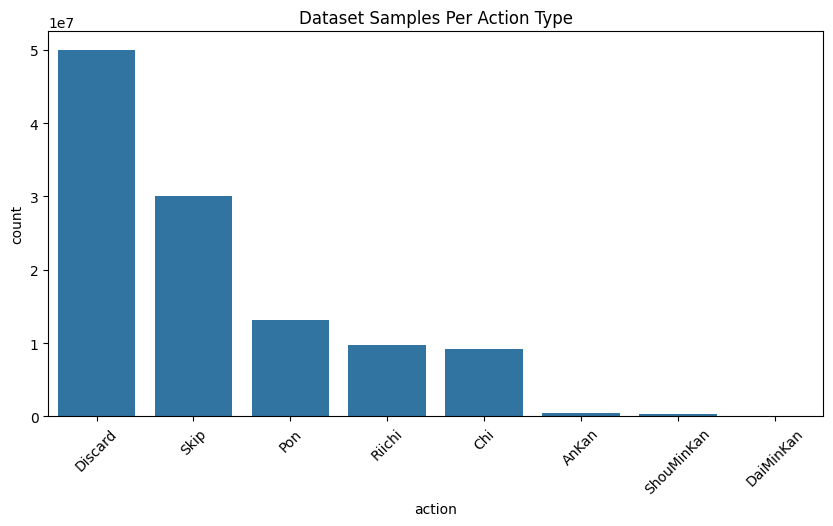
\includegraphics[width=0.8\textwidth]{figures/distribucion_acciones.png}
  \caption{Distribución de Número de Datos del Dataset por tipo de Acciones Válidas}
  \label{fig:dist_acciones_validas}
\end{figure}

En este gráfico se observa un fuerte desequilibrio entre los tipos de acciones. Los descartes son mucho más frecuentes que las llamadas o los distintos tipos de Kan, por lo que el presente trabajo se centra exclusivamente en los estados cuya acción observada es un descarte. El tratamiento conjunto de todas las decisiones requeriría considerar este desequilibrio y queda fuera del alcance del modelo desarrollado.

\subsection{Distribución de la Suma de Acciones Válidas de una Sample}

\begin{figure}[H]
  \centering
  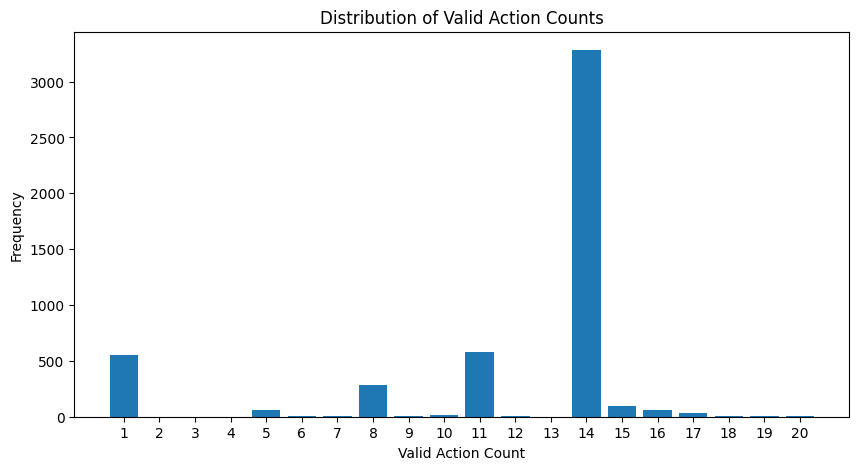
\includegraphics[width=0.8\textwidth]{figures/acciones_validas_dist.png}
  \caption{Distribución del número de acciones válidas del schema de Descarte}
  \label{fig:discard_valid_count}
\end{figure}

La mayor concentración ocurre en 14 acciones válidas, ya que una mano cerrada dispone normalmente de 14 fichas antes del descarte. También aparecen concentraciones en 11, 8 y 5 alternativas, asociadas a manos con una, dos o tres combinaciones abiertas, respectivamente, como se resume en la siguiente tabla:

\begin{table}[H]
  \centering
  \caption{Acciones válidas según melds abiertos}
  \label{tab:acciones_melds}
  \begin{tabular}{@{}cc@{}}
    \toprule
    \textbf{Acciones válidas} & \textbf{\textit{Melds} abiertos} \\
    \midrule
    11 & 1 \\
    8  & 2 \\
    5  & 3 \\
    2  & 4 \\
    \bottomrule
  \end{tabular}
\end{table}

Los estados con dos alternativas son menos frecuentes y suelen corresponder a manos con cuatro combinaciones ya formadas.

La base original contiene además numerosos estados con una única alternativa de descarte, situación habitual después de declarar \textit{Riichi}. Como en esos casos no existe una elección real entre varios descartes, se eliminaron para evitar que incrementasen artificialmente la precisión. La base filtrada conserva únicamente estados con más de una acción de tipo descarte.

Finalmente, el número de acciones válidas restante se explica debido a posibles acciones de \textit{Riichi} con diferentes piezas. 

\subsection{Frecuencia de Piezas Descartadas}

\begin{figure}[H]
  \centering
  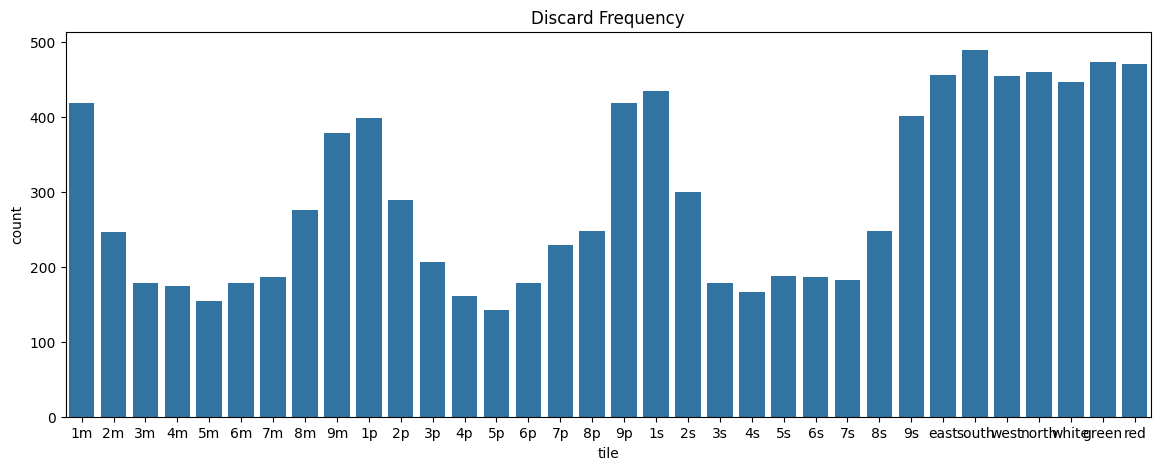
\includegraphics[width=0.8\textwidth]{figures/mostcommondiscarded.png}
  \caption{Frecuencia de las Piezas Descartadas}
  \label{fig:common_discarded}
\end{figure}

En este gráfico se observa que las fichas descartadas con mayor frecuencia son los honores (vientos y dragones), véase la Tabla \ref{tab:mahjong_tiles}, y las fichas terminales (unos y nueves). Una posible explicación es que, en muchas configuraciones de mano, estas fichas ofrecen menos posibilidades de formar secuencias que las fichas numeradas intermedias. Esta interpretación es descriptiva y no implica que deban descartarse siempre, ya que la decisión depende del estado concreto de la partida.

\subsection{Representación de un Estado}


Esta es la representación de un estado de mahjong dentro del Dataset:

\begin{lstlisting}[language=json, caption={Ejemplo de un estado}]
{
    {'round_wind': 0,
 'num_honba': 1,
 'num_riichi': 0,
 'player_wind': 0,
 'position': 0,
 'remain_tiles': 15,
 'dora_indicators': [7, 5],
 'hand_tiles': [1, 1, 2, 3, 3, 12, 13, 18, 19, 22, 22],
 'players': {'0': {'points': 41700,
   'riichi': False,
   'discards': [28, 27, 9, 16, 10, 6, 15, 20, 13, 32, 32, 0, 33, 33],
   'melds': [{'type': 2, 'tiles': [92, 98, 103, -1], 'who': [0, 0, 3, -1]}],
   'tsumo_giri': [0, 0, 0, 1, 0, 0, 1, 0, 0, 1, 1, 0, 0, 0]},
  '1': {'points': 19000,
   'riichi': False,
   'discards': [30, 27, 32, 18, 31, 17, 26, 26, 24, 2, 0, 14, 30, 10],
   'melds': [],
   'tsumo_giri': [0, 0, 0, 1, 0, 0, 0, 0, 1, 0, 1, 0, 0, 0]},
  '2': {'points': 20300,
   'riichi': False,
   'discards': [18, 17, 11, 16, 24, 25, 28, 23, 33, 32, 20, 7, 30, 17],
   'melds': [{'type': 5, 'tiles': [124, 126, 127, 125], 'who': [2, 2, 1, 2]},
    {'type': 2, 'tiles': [5, 13, 10, -1], 'who': [2, 2, 1, -1]}],
   'tsumo_giri': [0, 0, 0, 1, 0, 0, 0, 1, 0, 1, 1, 0, 1, 1]},
  '3': {'points': 19000,
   'riichi': False,
   'discards': [28, 29, 30, 18, 0, 11, 9, 27, 27, 0, 29, 26, 24, 25],
   'melds': [],
   'tsumo_giri': [0, 0, 0, 0, 0, 0, 1, 0, 0, 1, 1, 0, 0, 1]}},
 'valid_actions': [{'type': 1, 'tiles': [1], 'who': [0, -1, -1, -1]},
  {'type': 1, 'tiles': [1], 'who': [0, -1, -1, -1]},
  {'type': 1, 'tiles': [2], 'who': [0, -1, -1, -1]},
  {'type': 1, 'tiles': [3], 'who': [0, -1, -1, -1]},
  {'type': 1, 'tiles': [3], 'who': [0, -1, -1, -1]},
  {'type': 1, 'tiles': [12], 'who': [0, -1, -1, -1]},
  {'type': 1, 'tiles': [13], 'who': [0, -1, -1, -1]},
  {'type': 1, 'tiles': [18], 'who': [0, -1, -1, -1]},
  {'type': 1, 'tiles': [19], 'who': [0, -1, -1, -1]}],
 'action_idx': 7}
}
\end{lstlisting}

De este registro se obtiene la siguiente información:

\begin{table}[H]
  \centering
  \caption{Campos de un Estado de Mahjong}
  \label{tab:state_fields}
  \begin{tabular}{@{}clp{8cm}@{}}
    \toprule
    \textbf{Campo} & \textbf{Tipo} & \textbf{Descripción} \\
    \midrule
    round\_wind & int & Identificador de ronda utilizado por el dataset \\
    num\_honba & int & Número de honba \\
    num\_riichi & int & Número de riichi's (0-3) \\
    player\_wind & int & Viento del jugador (0-3) \\
    position & int & Posición del jugador (0-3) \\
    remain\_tiles & int & Número de fichas restantes en el muro (0-70) \\
    dora\_indicators & list[int] & Indicadores de dora en codificación Tenhou (0-135) \\
    hand\_tiles & list[int] & Fichas de la mano en codificación Tenhou (0-135) \\
    players & dict[int, dict] & Información de los jugadores, incluyendo puntos, riichi, descartes, melds y tsumo\_giri. \\
    valid\_actions & list[dict] & Lista de acciones válidas para el jugador actual. \\
    action\_idx & int & Índice de la acción tomada por el jugador actual. \\
    \bottomrule
  \end{tabular}
\end{table}

De estos datos, podemos aún extraer los campos de players:

\begin{table}[H]
  \centering
  \caption{Campos de un Jugador en un Estado de Mahjong}
  \label{tab:player_fields}
  \begin{tabular}{@{}clp{8cm}@{}}
    \toprule
    \textbf{Campo} & \textbf{Tipo} & \textbf{Descripción} \\
    \midrule
    points & int & Puntos del jugador (0-50000) \\
    riichi & bool & Indica si el jugador ha declarado riichi (True/False) \\
    discards & list[int] & Lista de fichas descartadas por el jugador (0-33) \\
    melds & list[dict] & Lista de combinaciones del jugador, cada una con tipo, fichas y procedencia. \\
    tsumo\_giri & list[int] & Lista indicando si cada ficha fue descartada inmediatamente después de ser robada (1) o no (0). \\
    \bottomrule
  \end{tabular}
\end{table}

Campos de melds:

\begin{table}[H]
  \centering
  \caption{Campos de un Meld en un Estado de Mahjong}
  \label{tab:meld_fields}
  \begin{tabular}{@{}clp{8cm}@{}}
    \toprule
    \textbf{Campo} & \textbf{Tipo} & \textbf{Descripción} \\
    \midrule
    type & int & Tipo de meld (2: Pon, 3: Chii, 4: DaiMinKan, 5: ShouMinKan, 6: AnKan) \\
    tiles & list[int] & Fichas que componen el meld en codificación Tenhou (0-135) \\
    who & list[int] & Lista indicando quién contribuyó a cada ficha del meld (-1 para fichas propias, 0-3 para otros jugadores) \\
    \bottomrule
  \end{tabular}
\end{table}

Y, por fin, campos de valid\_actions:

\begin{table}[H]
  \centering
  \caption{Campos de una Acción Válida en un Estado de Mahjong}
  \label{tab:valid_action_fields}
  \begin{tabular}{@{}clp{8cm}@{}}
    \toprule
    \textbf{Campo} & \textbf{Tipo} & \textbf{Descripción} \\
    \midrule
    type & int & Tipo de acción (0: Skip, 1: Discard, 2: Chi, 3: Pon, 4: DaiMinKan, 5: ShouMinKan, 6: AnKan, 7: Riichi, 8: Ron, 9: Tsumo, 10: Kyushukyuhai, 11: Chankan) \\
    tiles & list[int] & Fichas involucradas en la acción en codificación Tenhou (0-135) \\
    who & list[int] & Lista indicando quién realiza la acción y quién contribuye a ella (-1 para el jugador actual, 0-3 para otros jugadores) \\
    \bottomrule
  \end{tabular}
\end{table}


\section{Arquitectura del Modelo}
\label{sec:model-architecture}

Como se explicó en la Subsección \ref{subsec:transformer}, el modelo desarrollado en este trabajo utiliza una arquitectura basada en el codificador de un Transformer. La elección de una arquitectura de tipo \textit{encoder-only} se debe a que el objetivo del sistema no consiste en generar una secuencia de salida, sino en analizar la representación disponible de un estado de Riichi Mahjong y puntuar las acciones candidatas proporcionadas por el dataset.

La Figura \ref{fig:model-architecture} muestra el flujo general de procesamiento, desde la normalización de la instantánea almacenada en el conjunto de datos hasta la predicción final realizada por el modelo.

\begin{figure}[H]
    \centering

    \begin{tikzpicture}[
        node distance=0.55cm,
        font=\small,
        >=Latex,
        block/.style={
            rectangle,
            rounded corners=2mm,
            draw=black!65,
            line width=0.7pt,
            align=center,
            minimum height=1.05cm,
            text width=6.2cm,
            fill=black!3
        },
        process/.style={
            block,
            fill=blue!7
        },
        neural/.style={
            block,
            fill=orange!10
        },
        output/.style={
            block,
            fill=green!10
        },
        arrow/.style={
            ->,
            line width=0.8pt,
            draw=black!70
        },
        annotation/.style={
            font=\scriptsize,
            text=black!65,
            align=center
        }
    ]

    % Entrada y procesamiento
    \node[block] (raw) {
        \textbf{Datos de Tenhou}\\
        Estado almacenado en la base de datos
    };

    \node[process, below=of raw] (parser) {
        \textbf{Normalización del estado}\\
        Mano, descartes, melds, dora, vientos y contexto de la ronda
    };

    \node[process, below=of parser] (tokens) {
        \textbf{Tokenización}\\
        Conversión del estado canónico en una secuencia de identificadores
    };

    % Representación
    \node[neural, below=of tokens] (embedding) {
        \textbf{Capa de embeddings}\\
        Proyección de cada token a un vector continuo de dimensión $d_{\text{model}}$
    };

    \node[neural, below=of embedding] (encoder) {
        \textbf{Transformer Encoder}\\
        Self-attention multi-cabeza, red feed-forward, conexiones residuales
        y normalización
    };

    \node[neural, below=of encoder] (context) {
        \textbf{Representación contextualizada}\\
        Integración de las relaciones entre los elementos del estado
    };

    % Salida
    \node[output, below=of context] (policy) {
        \textbf{Cabeza de política}\\
        Capa lineal que asigna una puntuación a cada acción candidata
    };


    \node[output, below=of policy] (prediction) {
        \textbf{Predicción del descarte}\\
        Selección de la acción legal con mayor puntuación
    };

    % Flechas
    \draw[arrow] (raw) -- (parser);
    \draw[arrow] (parser) -- (tokens);
    \draw[arrow] (tokens) -- (embedding);
    \draw[arrow] (embedding) -- (encoder);
    \draw[arrow] (encoder) -- (context);
    \draw[arrow] (context) -- (policy);
    \draw[arrow] (policy) -- (prediction);

    % Agrupaciones laterales
    \begin{scope}[on background layer]
        \node[
            draw=blue!45,
            dashed,
            rounded corners=3mm,
            fit=(parser)(tokens),
            inner sep=0.18cm,
            label={[annotation]right:Preprocesamiento}
        ] {};

        \node[
            draw=orange!55,
            dashed,
            rounded corners=3mm,
            fit=(embedding)(encoder)(context),
            inner sep=0.18cm,
            label={[annotation]right:Modelo neuronal}
        ] {};

        \node[
            draw=green!45!black,
            dashed,
            rounded corners=3mm,
            fit=(policy)(prediction),
            inner sep=0.18cm,
            label={[annotation]right:Selección de la acción}
        ] {};
    \end{scope}

    \end{tikzpicture}

    \caption{Flujo de procesamiento y arquitectura del modelo propuesto.}
    \label{fig:model-architecture}
\end{figure}

\subsection{Reconstrucción del estado de juego}

Los registros del conjunto de datos no pueden utilizarse directamente como entrada de una red neuronal, ya que contienen la información de la partida en un formato estructurado que debe ser interpretado y normalizado previamente.

Por este motivo, se desarrolló un proceso de normalización encargado de transformar cada instantánea del dataset en una representación canónica. Esta representación intermedia reúne la mano del jugador, los descartes visibles, las combinaciones abiertas, los indicadores de Dora, los vientos y otros elementos contextuales. No reconstruye la partida desde un registro de eventos ni recupera información oculta.


\subsection{Tokenización del estado}

Una vez normalizada la instantánea, su información se transforma en una secuencia de tokens mediante un tokenizador desarrollado específicamente para este proyecto.

Cada token representa una unidad semántica del estado de juego. Se crean tokens para la mano, los descartes, las combinaciones, las acciones candidatas y ciertos elementos contextuales. Sin embargo, como se detalla más adelante, la implementación final solo tensoriza una parte de los metadatos almacenados en estos objetos intermedios.

Esta representación simbólica se eligió como alternativa a las codificaciones espaciales empleadas por modelos basados en redes convolucionales. En lugar de transformar el estado del Mahjong en una estructura bidimensional similar a una imagen, la tokenización permite representar sus componentes de forma explícita y compacta.

La secuencia resultante mantiene diferenciada la naturaleza de cada elemento del estado y facilita la incorporación de nueva información sin necesidad de rediseñar completamente la estructura de entrada.

\subsection{Capa de embeddings}

Los identificadores discretos obtenidos durante la tokenización no pueden ser procesados directamente por el Transformer. Por ello, cada token se proyecta a un vector continuo de dimensión fija mediante una capa de embeddings entrenable.

Durante el entrenamiento, el modelo ajusta estas representaciones para capturar relaciones entre los distintos elementos del estado. De esta forma, tokens asociados a fichas, zonas del tablero o situaciones estratégicas relacionadas pueden adquirir representaciones útiles para la predicción.

La salida de esta etapa es una matriz de vectores, donde cada fila corresponde a la representación numérica de uno de los tokens del estado.

\subsection{Transformer Encoder}

La secuencia de embeddings se introduce posteriormente en un Transformer Encoder. Este bloque está compuesto por varias capas que combinan mecanismos de \textit{multi-head self-attention}, redes neuronales \textit{feed-forward}, conexiones residuales y normalización.

El mecanismo de autoatención permite que cada elemento de la entrada tenga en cuenta la información proporcionada por el resto de tokens. En la implementación final, el modelo relaciona principalmente las fichas de la mano, los descartes visibles, el tipo y propietario de las combinaciones y las acciones candidatas. Otros campos contextuales permanecen en la representación intermedia, pero no se incorporan aún al tensor de entrada.

Por tanto, la salida del codificador no representa cada token de forma aislada, sino contextualizada respecto a la información que efectivamente recibe el modelo.

\subsection{Cabeza de política y acciones legales}

La representación contextual producida por el Transformer se utiliza para asignar una puntuación a las acciones de descarte disponibles. Esta parte final del modelo recibe el nombre de cabeza de política o \textit{policy head}.

Para cada muestra se utiliza el conjunto de acciones candidatas proporcionado por el dataset. Aunque la acción objetivo de todos los registros de la tabla \textit{Discard} es un descarte, algunos estados incluyen además candidatos de Riichi o Kan. La cabeza de política calcula un valor o \textit{logit} para cada candidato. Como su número puede variar entre estados, la salida del modelo también presenta una longitud variable.

La acción predicha corresponde al descarte con mayor puntuación:

\begin{equation}
    \hat{a} = \arg\max_{a \in A(s)} z_a,
\end{equation}

donde $A(s)$ representa el conjunto de acciones candidatas para el estado $s$ y $z_a$ el logit asignado por la cabeza de política a la acción $a$.

Durante el entrenamiento, los logits generados por el modelo se comparan con la acción observada en el dataset mediante una función de pérdida de entropía cruzada (\textit{Cross-Entropy Loss})\cite{goodfellow2016deep}. Esta función aplica internamente una normalización Softmax sobre los logits para obtener una distribución de probabilidad y penaliza aquellas predicciones que asignan una baja probabilidad a la acción objetivo. Como consecuencia, el modelo aprende progresivamente a incrementar la puntuación de las decisiones observadas en el conjunto de entrenamiento.

\subsection{Justificación de las decisiones arquitectónicas}

La arquitectura fue diseñada atendiendo tanto a las características del problema como a los recursos disponibles para el desarrollo del proyecto.

En primer lugar, se eligió un Transformer Encoder porque el problema se formula como una tarea de clasificación condicionada por una representación del estado observable. No es necesario generar una secuencia ni predecir estados futuros, por lo que una arquitectura \textit{encoder-decoder} introduciría complejidad adicional sin aportar una ventaja directa para este objetivo.

En segundo lugar, la representación mediante tokens permite mantener una correspondencia clara entre los elementos del estado y la información procesada por el modelo. Esta decisión mejora la interpretabilidad del preprocesamiento y evita la necesidad de construir una representación espacial específica para redes convolucionales.

Finalmente, la predicción se limita a las acciones legales de cada estado. Esta elección evita que el modelo tenga que asignar probabilidad a descartes imposibles y adapta la salida a la naturaleza variable de las decisiones disponibles en una partida de Mahjong.

En conjunto, la arquitectura propuesta busca alcanzar un equilibrio entre capacidad de representación, coste computacional y claridad de implementación.


\subsection{Diseño conceptual de la tokenización}
\label{subsec:tokenization}

Durante el diseño se definieron las siguientes categorías de información. Esta sección documenta la representación semántica intermedia y las alternativas consideradas; no todos sus campos fueron incorporados finalmente a los embeddings utilizados por los checkpoints.

\begin{table}[H]
  \centering
  \begin{tabular}{|l|l|l|l|l|}
    \hline
    \textbf{Categoria} & \textbf{Ejemplos} & \textbf{Ordenado} & \textbf{Público} & \textbf{Dinámico} \\
    \hline
    \hline
    Piezas de mano & 5m, este & No & No & Sí \\
    \hline
    Descartes & descarte 9m & Sí & Sí & Sí \\
    \hline
    Melds & pon/chi/kan & Parcialmente  & Sí & Sí \\
    \hline
    Acciones candidatas & descartar 5m & No & N/A & Sí
    \\
    \hline
    Contexto & Viento de la Ronda & No & Sí & Lento
    \\
    \hline
    Estatus de los jugadores & riichi, puntos & No & Sí & Sí \\
    \hline
  \end{tabular}
  \caption{Categorías de Informaciones}
  \label{tab:catinfo}
\end{table}

Un estado de Mahjong se representa como una colección de tokens semánticos. Cada token representa una categoría diferente de información de juego y puede contener metadatos asociados.

A continuación veremos, para cada categoría, cuáles son los campos que tendrá el token.

\subsubsection{Tokens de Mano}

Las piezas de la mano representan la identidad de la pieza, una distinción entre duplicados (qué copia de la pieza es) y un indicador de si se trata de una Dora roja.

\begin{table}[H]
  \centering
  \begin{tabular}{|l|l|}
  \hline
  \textbf{Campo} & \textbf{Objetivo}         \\ \hline
  token\_type    & identifica el token HAND    \\ \hline
  tile\_type     & pieza de Mahjong    \\ \hline
  copy\_index    & diferencia copias de piezas \\ \hline
  is\_red        & soporte de dora rojo        \\ \hline
  \end{tabular}
  \caption{Campos de Token de Mano}
  \label{tab:hand_token}
\end{table}

\subsubsection{Tokens de Descarte}

Los tokens de descarte representan eventos públicos y ordenados. Los campos de un token de descarte son los siguientes:

\begin{table}[H]
  \centering
  \begin{tabular}{|l|l|}
  \hline
  \textbf{Campo} & \textbf{Objetivo}         \\ \hline
  token\_type    & identifica el token DISCARD    \\ \hline
  player & jugador que ha descartado la pieza \\ \hline
  tile\_type     & pieza de Mahjong    \\ \hline
  copy\_index    & diferencia copias de piezas \\ \hline
  is\_red        & soporte de dora rojo        \\ \hline
  is\_tsumogiri & si la pieza descartada fue la ficha recién robada \\ \hline
  is\_riichi\_declaration & si al descartar esa pieza se declara riichi \\ \hline
  global\_order & orden cronológico del descarte en la ronda \\ \hline
  player\_discard\_order & índice de descarte para el jugador \\ \hline
  \end{tabular}
  \caption{Campos de Token de Descarte}
  \label{tab:discard_token}
\end{table}


\subsubsection{Tokens de Melds}

Los Tokens de Melds representan eventos de melds que son públicos y ordenados, los campos de un token de meld son los siguientes:

\begin{table}[]
\centering
\begin{tabular}{|l|l|}
\hline
\textbf{Campo}  & \textbf{Objetivo}                            \\ \hline
token\_type     & identifica el token MELD                    \\ \hline
player          & jugador que posee el meld                   \\ \hline
meld\_type      & chi / pon / kan                             \\ \hline
tile\_types     & piezas que componen el meld                 \\ \hline
copy\_indices   & distinción entre duplicados                 \\ \hline
red\_flags      & soporte de dora rojo                        \\ \hline
source\_players & jugadores que contribuyeron para cada pieza \\ \hline
global\_order   & orden cronológico de la llamada             \\ \hline
\end{tabular}
\caption{Campos de Token de Melds}
\label{tab:melds_token}
\end{table}


\subsubsection{Tokens de Acciones}

Los Tokens de Acciones representan eventos de acciones candidatas que son públicos y ordenados, los campos de un token de acción son los siguientes:

\begin{table}[H]
  \centering
  \begin{tabular}{|l|l|}
    \hline
    \textbf{Campo} & \textbf{Objetivo}         \\ \hline
    token\_type    & identifica el token ACTION    \\ \hline
    acting\_player & jugador que realiza la acción \\ \hline
    action\_index  & índice dentro del conjunto de candidatos legales \\ \hline
    action\_type   & descartar / riichi / pon / etc \\ \hline
    tile\_types    & piezas involucradas en la acción \\ \hline
    copy\_indices  & distinción de duplicados \\ \hline
    red\_flags     & soporte de dora rojo \\ \hline
    source\_players & fuente de las piezas llamadas \\ \hline
    global\_order  & orden cronológico de la acción \\ \hline
  \end{tabular}
  \caption{Campos de Token de Acciones}
  \label{tab:action_token}
  
\end{table}

\subsubsection{Tokens de Estado de Juego}

Los Tokens de Estado de Juego representan información contextual del juego que es pública y no ordenada, los campos de un token de estado de juego son los siguientes:


\begin{table}[H]
  \centering
  \begin{tabular}{|l|l|}
    \hline
    \textbf{Campo} & \textbf{Objetivo}         \\ \hline
    token\_type    & identifica el token GAME\_STATE    \\ \hline
    round\_wind      & ronda Este/Sur            \\ \hline
    honba\_count     & honba actual               \\ \hline
    riichi\_sticks   & depósitos de riichi             \\ \hline
    remaining\_tiles  & piezas restantes en la pared          \\ \hline
    dora\_indicators & indicadores de dora actuales     \\ \hline
  \end{tabular}
  \caption{Campos de Token de Estado de Juego}
  \label{tab:game_state_token}
\end{table}

\subsubsection{Tokens de Estado de Jugadores}

Los Tokens de Estado de Jugadores representan información contextual de cada jugador que es pública y no ordenada, los campos de un token de estado de jugadores son los siguientes:


\begin{table}[H]
  \centering
  \begin{tabular}{|l|l|}
    \hline
    \textbf{Campo} & \textbf{Objetivo}         \\ \hline
    token\_type    & identifica el token PLAYER\_STATE    \\ \hline
    player          & identidad del jugador                   \\ \hline
    seat\_wind      & este/sur/oeste/norte          \\ \hline
    score           & puntos actuales                 \\ \hline
    riichi\_status  & si el jugador ha declarado riichi \\ \hline
    placement       & posición actual                \\ \hline
    open\_hand      & si el jugador tiene mano abierta \\ \hline
  \end{tabular}
  \caption{Campos de Token de Estado de Jugadores}
  \label{tab:player_state_token}
\end{table}

\subsection{Diseño conceptual del embedding}

Inicialmente se planteó una composición de embeddings semánticos y de metadatos con la siguiente estructura general:

$$\text{Embedding}(\text{token}) = 
\text{token\_type\_embedding} +
\text{semantic\_embedding} +
\text{metadata\_embedding} +
\text{positional\_embeddings} $$

Los distintos tipos de tokens utilizarían diferentes embeddings en función de su estructura semántica.

Cada categoría de token tendrá un embedding dedicado de tipo de token, que podrá ser uno de los siguientes: HAND, DISCARD, MELD, ACTION, GAME\_STATE o PLAYER\_STATE.

A continuación se documentan las combinaciones consideradas para cada token semántico. Estas expresiones pertenecen al diseño conceptual; la Subsección siguiente describe la implementación que se utilizó realmente para entrenar y evaluar los modelos.

\subsubsection{Embedding de Tokens de Piezas}

Este embedding codifica la identidad de la pieza, por ejemplo:
1m, 5p, east, red\_dragon. Los embeddings de piezas son compartidos entre los tokens de mano, descarte, melds y de acciones.

\subsubsection{Embedding del índice de copia}

Instancias de piezas duplicadas (por ejemplo, dos 5m) se distinguen mediante un índice de copia. Este embedding permite al modelo diferenciar entre estas instancias. 

\subsubsection{Embedding de Jugador}

Este embedding codifica la identidad del jugador, por ejemplo, jugador 0, jugador 1, etc. Los embeddings de jugadores son compartidos entre los tokens de descarte, melds, acciones y estado de jugadores.


\subsubsection{Embeddings Posicionales}

Los embeddings posicionales preservan el orden temporal de eventos como los descartes, el momento en que se realizaron los melds y la secuencia de acciones. Se plantearon dos esquemas posicionales: el orden cronológico global y el orden local de descartes de cada jugador.

\subsubsection{Embeddings de Metadatos}

Los embeddings de metadatos codifican información adicional relevante para cada token, como indicadores de dora, estado de riichi, y otros atributos contextuales. Estos embeddings permiten al modelo capturar relaciones complejas entre los tokens y el contexto del juego.

\subsubsection{Embedding de Token de Mano}

Los tokens de mano representan piezas escondidas del jugador actual y es definida por la siguiente estructura de embedding:


$$\text{E\_hand} = \text{E\_token\_type} + \text{E\_tile} + \text{E\_copy} + \text{E\_red}$$

Dónde:

\begin{itemize}
  \item E\_token\_type identifica el token como una entidad de tipo HAND,
  \item E\_tile representa la identidad semántica de la pieza,
  \item E\_copy distingue entre instancias duplicadas de piezas,
  \item E\_red indica si la pieza es un dora rojo.
\end{itemize}

\subsubsection{Embedding de Token de Descarte}

Los tokens de descarte representan eventos de descartes que son públicos y ordenados, y su embedding es definido por la siguiente estructura:

\begin{equation}
  \begin{split}
    \text{E\_discard} = \text{E\_token\_type} + \text{E\_tile} + \text{E\_copy} + \\ \text{E\_red} + \text{E\_player} + \text{E\_tsumogiri} + \\ \text{E\_riichi\_declaration} + \text{E\_global\_position} + \text{E\_local\_position}
  \end{split}
\end{equation}

Dónde:

\begin{itemize}
  \item E\_token\_type identifica el token como una entidad de tipo DISCARD,
  \item E\_tile representa la identidad semántica de la pieza,
  \item E\_copy distingue entre instancias duplicadas de piezas,
  \item E\_red indica si la pieza es un dora rojo,
  \item E\_player identifica al jugador que ha descartado la pieza,
  \item E\_tsumogiri indica si la ficha descartada fue la ficha recién robada,
  \item E\_riichi\_declaration indica si al descartar esa pieza se declara riichi,
  \item E\_global\_position representa el orden cronológico global del descarte,
  \item E\_local\_position representa el orden de descarte relativo al jugador.
\end{itemize}

\subsubsection{Embedding de Token de Meld}

Tokens de Melds representan llamadas hechas durante la partida, y su embedding es definido por la siguiente estructura:

\begin{equation}
  \begin{split}
    \text{E\_meld} = \text{E\_token\_type} + \text{E\_player} + \text{E\_meld\_type} + \\ \text{E\_tile\_set} + \text{E\_copy\_set} + \text{E\_red\_set} + \\ \text{E\_source\_players} + \text{E\_global\_position}
  \end{split}
\end{equation}


Dónde:

\begin{itemize}
  \item E\_token\_type identifica el token como una entidad de tipo MELD,
  \item E\_player identifica al jugador que posee el meld,
  \item E\_meld\_type representa el tipo de meld (chi, pon, kan, etc),
  \item E\_tile\_set codifica las piezas que componen el meld,
  \item E\_copy\_set distingue entre instancias duplicadas de piezas,
  \item E\_red\_set codifica la información de dora rojo,
  \item E\_source\_players identifica los jugadores que contribuyeron a cada pieza del meld,
  \item E\_global\_position representa el orden cronológico de la llamada.
\end{itemize}

\subsubsection{Embedding de Token de Acción}

Tokens de Acciones representan eventos de acciones candidatas que son públicos y ordenados, y su embedding es definido por la siguiente estructura:

\begin{equation}
  \begin{split}
    \text{E\_action} = \text{E\_token\_type} + \text{E\_action\_type} + \\ \text{E\_tile\_set} + \text{E\_copy\_set} + \text{E\_red\_set} + \\ \text{E\_source\_players} + \text{E\_global\_position}
  \end{split}
\end{equation}


Dónde:

\begin{itemize}
  \item E\_token\_type identifica el token como una entidad de tipo ACTION,
  \item E\_action\_type representa descarte, riichi, chi, pon, kan, etc,
  \item E\_tile\_set representa las piezas involucradas en la acción,
  \item E\_copy\_set distingue entre instancias duplicadas de piezas,
  \item E\_red\_set codifica la información de dora rojo,
  \item E\_source\_players identifica las fuentes de las piezas para llamadas,
  \item E\_global\_position representa el timing de la acción.
\end{itemize}

\subsubsection{Embedding de Token de Estado de Juego}

Tokens de Estado de Juego representan información contextual del juego que es pública y no ordenada, y su embedding es definido por la siguiente estructura:

\begin{equation}
  \begin{split}
    \text{E\_game} = \text{E\_token\_type} + \text{E\_round} + \text{E\_honba} + \\ \text{E\_riichi\_sticks} + \text{E\_remaining\_tiles} + \text{E\_dora\_set}
  \end{split}
\end{equation}

Dónde:

\begin{itemize}
  \item E\_token\_type identifica el token como una entidad de tipo GAME\_STATE,
  \item E\_round codifica el viento de la ronda (este/sur),
  \item E\_honba representa el número de honba actuales,
  \item E\_riichi\_sticks codifica la cantidad de depósitos de riichi,
  \item E\_remaining\_tiles representa las piezas restantes en la pared,
  \item E\_dora\_set codifica los indicadores de dora actuales.
\end{itemize}

\subsubsection{Embedding de Token de Estado de Jugador}

El Token de Estado de Jugador representa información contextual persistente asociada con cada jugador, y su embedding es definido por la siguiente estructura:


\begin{equation}
  \begin{split}
    \text{E\_player\_state} = \text{E\_token\_type} + \text{E\_player} + \\ \text{E\_seat} + \text{E\_score} + \text{E\_riichi\_status} + \text{E\_open\_hand}
  \end{split}
\end{equation}

Dónde:

\begin{itemize}
  \item E\_token\_type identifica el token como una entidad de tipo PLAYER\_STATE,
  \item E\_player codifica la identidad del jugador,
  \item E\_seat representa el viento de asiento del jugador (este/sur/oeste/norte),
  \item E\_score codifica los puntos actuales del jugador,
  \item E\_riichi\_status indica si el jugador ha declarado riichi,
  \item E\_open\_hand indica si el jugador tiene una mano abierta.
\end{itemize}

\subsection{Tensorización y embeddings implementados}

La implementación final transforma cada token en seis identificadores discretos: tipo de token, tipo de ficha, índice de copia, jugador, tipo de acción y posición absoluta dentro de la secuencia. Cada identificador dispone de una tabla de embeddings entrenable de dimensión 128. La representación de entrada se obtiene sumando los seis vectores:

\begin{equation}
E = E_{\text{tipo}} + E_{\text{ficha}} + E_{\text{copia}} + E_{\text{jugador}} + E_{\text{acción}} + E_{\text{posición}}.
\end{equation}

La información tensorizada depende de la categoría del token. Los tokens de mano incorporan el tipo y la copia física de la ficha. Los descartes incorporan tipo de ficha, copia y jugador. Los melds incorporan el jugador propietario y el tipo de llamada, mientras que las acciones candidatas incorporan el tipo de acción y la primera ficha asociada. Todos los tokens reciben, además, su tipo y su posición absoluta en la secuencia.

Algunos metadatos presentes en las clases semánticas no se trasladan todavía a estos identificadores. Entre ellos se encuentran la condición de dora roja, el indicador de \textit{tsumogiri}, la declaración de Riichi asociada a un descarte, las fichas y procedencias completas de los melds, los puntos, el estado de Riichi de cada jugador, el número de honba, los depósitos de Riichi, las fichas restantes y los indicadores de Dora. En particular, los tokens \texttt{GAME\_STATE} y \texttt{PLAYER\_STATE} conservan su tipo y posición, pero sus demás atributos no se codifican en la entrada de los checkpoints evaluados.

Esta diferencia entre el diseño conceptual y la versión implementada constituye una limitación de la representación actual. Su incorporación requeriría ampliar el tensorizador y volver a entrenar los modelos, por lo que se plantea como trabajo futuro y no se atribuye a los resultados presentados.

\subsection{Configuración final del modelo}

Los dos modelos comparados utilizan una dimensión de embedding de 128, ocho cabezas de atención, cuatro capas de Transformer Encoder, una dimensión de 512 en la red \textit{feed-forward} y un \textit{dropout} de 0,1. La cabeza de política consiste en una capa lineal que transforma el estado oculto de cada token de acción en un único logit. En total, la arquitectura contiene 867.073 parámetros entrenables.
